\documentclass[12pt, a4paper, oneside]{ctexart}
\usepackage{amsmath, amsthm, amssymb, bm, color, framed, graphicx, hyperref, mathrsfs, mathtools, enumerate, tikz}
\usepackage{float}
\usepackage{booktabs}
\usepackage{subcaption} 



\usetikzlibrary{patterns}

\title{\textbf{Homework 12}}
\author{萃英学院\qquad 2022级\qquad 王一鑫}
\date{\today}
\linespread{1.5}
\newcounter{problemname}
\newenvironment{problem}{\begin{framed}\stepcounter{problemname}\par\noindent\textsc{Problem \arabic{problemname}. }}{\end{framed}\par}
\newenvironment{solution}{%
	\par\noindent\textsc{Solution. }\ignorespaces
}{%
	\hfill$\qed$\par
}
\newenvironment{note}{\par\noindent\textsc{Note of Problem \arabic{problemname}. }}{\\\par}

\begin{document}
	
	\maketitle
	
	
	\begin{problem}
		(Exercise 6.16)
		
		Verify Corollary 6.8 for each of the following graphs:
		\begin{enumerate}[(i)]
			\item \(K_{3,5}\);
			\item \(K_{3,3,3}\);
			\item the graph of the octahedron.
		\end{enumerate}
		
	\end{problem}
	
	\begin{solution}
		\begin{enumerate}[(i)]
			
			\item It is a classical result that the connectivity \(\kappa(K_{m,n})\) of a complete bipartite graph \(K_{m,n}\) is equal to the minimum of \(m\) and \(n\); that is, \(\kappa(K_{m,n}) = \min(m,n)\). Therefore, for \(K_{3,5}\), we have \(\kappa(K_{3,5}) = 3\). According to the definition of \(k\)-connectivity, we must verify that any two distinct vertices in \(K_{3,5}\) are connected by at least 3 vertex-disjoint paths. For any two vertices in the same partition, they are connected through all the vertices of the opposite partition, providing exactly 3 vertex-disjoint paths. For vertices in different partitions, they are directly connected by an edge, and there exist multiple alternative paths using the vertices in the remaining partitions, ensuring the existence of at least 3 vertex-disjoint paths. Thus, \(K_{3,5}\) satisfies Corollary 6.8.
			
			\item For complete tripartite graphs \(K_{r,r,r}\), it is known that the connectivity is given by \(\kappa(K_{r,r,r}) = 2r\). Hence, for \(K_{3,3,3}\), we have \(\kappa(K_{3,3,3}) = 6\). To satisfy Corollary 6.8, we must show that any two distinct vertices in \(K_{3,3,3}\) are connected by at least 6 vertex-disjoint paths. Consider any pair of vertices. If both vertices lie in the same partition, they are connected through the remaining two partitions, each contributing at least 3 internally disjoint paths, for a total of at least 6 vertex-disjoint paths. If the vertices are in different partitions, the third partition provides 3 vertex-disjoint paths, and the remaining vertices from the other partitions contribute additional disjoint paths, ensuring a total of 6 vertex-disjoint paths. Therefore, \(K_{3,3,3}\) satisfies Corollary 6.8.
			\item The octahedron graph has 6 vertices and 12 edges and is the skeleton of the regular octahedron. It is a well-known result that the connectivity of the octahedron graph is \(\kappa = 4\). We must demonstrate that for any two distinct vertices, there exist at least 4 vertex-disjoint paths between them. Since the octahedron is a 4-connected graph, Menger's theorem guarantees that for any two vertices, there exist at least 4 vertex-disjoint paths connecting them. This directly verifies Corollary 6.8 for the octahedron graph.
		\end{enumerate}
		
	\end{solution}
	
	\begin{problem}
		(Exercise 6.17)
		
		Verify Theorem 6.9 for each graph in Fig \ref{fig:1}.
					\begin{figure}[H]
							\small
							\centering
							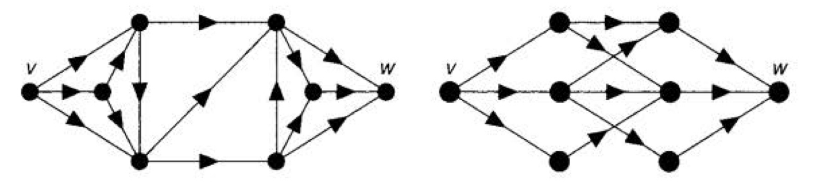
\includegraphics[width=0.8\columnwidth]{Figure/Fig1.png}
							\caption{Figure for Problem 2.}
							\label{fig:1}
						\end{figure}
	\end{problem}
	
	\begin{solution}
		There are three arc-disjoint paths from v to w, and three arcs in a vw-disconnecting set, shown in Fig \ref{fig:2}.
		\begin{figure}[H]
			\small
			\centering
			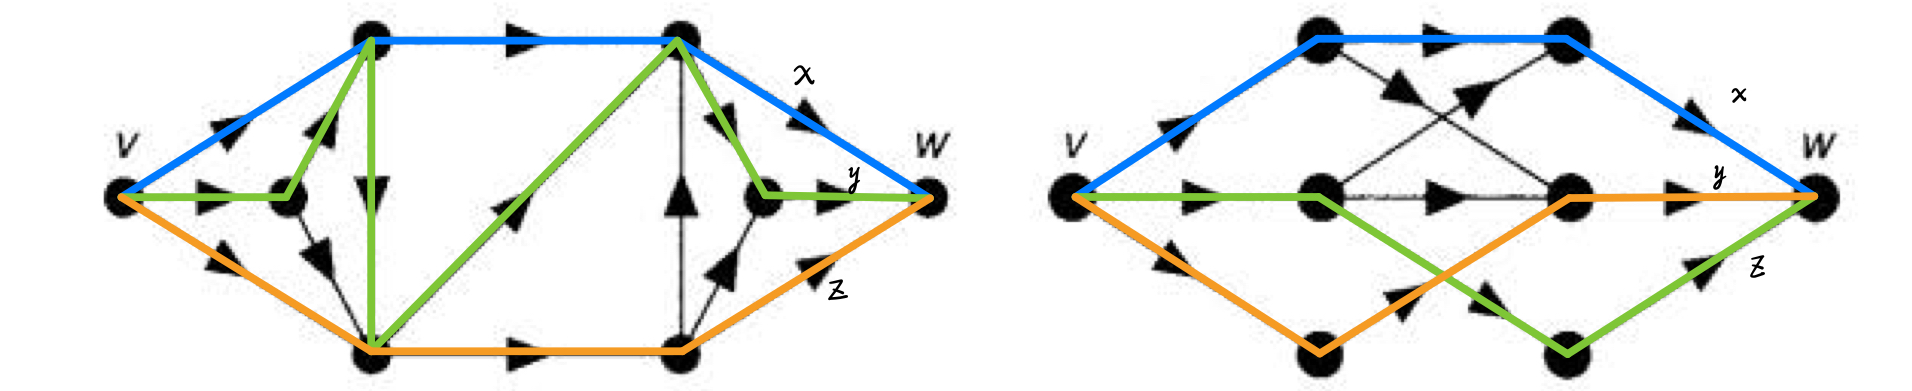
\includegraphics[width=0.8\columnwidth]{Figure/Fig2.jpg}
			\caption{Figure for Problem 2.}
			\label{fig:2}
		\end{figure}
	\end{solution}
	
	\begin{problem}
		(Exercise 6.21)
		
		Find a flow with value 20 in the network of Fig \ref{fig:3} . Is it a maximum flow?
		\begin{figure}[H]
			\small
			\centering
			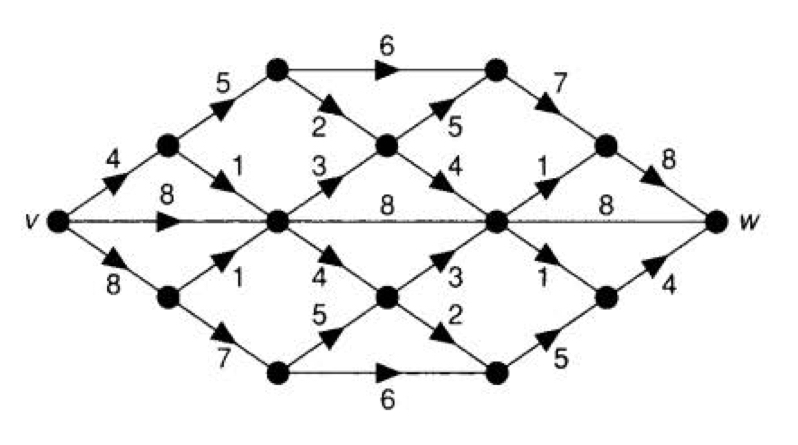
\includegraphics[width=0.8\columnwidth]{Figure/Fig3.jpg}
			\caption{Figure for Problem 3.}
			\label{fig:3}
		\end{figure}
	\end{problem}
	
	\begin{solution} 
		
		By the construction of flow-augmenting paths, I find a flow with value 20 shown in Fig \ref{fig:4}.
		\begin{figure}[H]
			\small
			\centering
			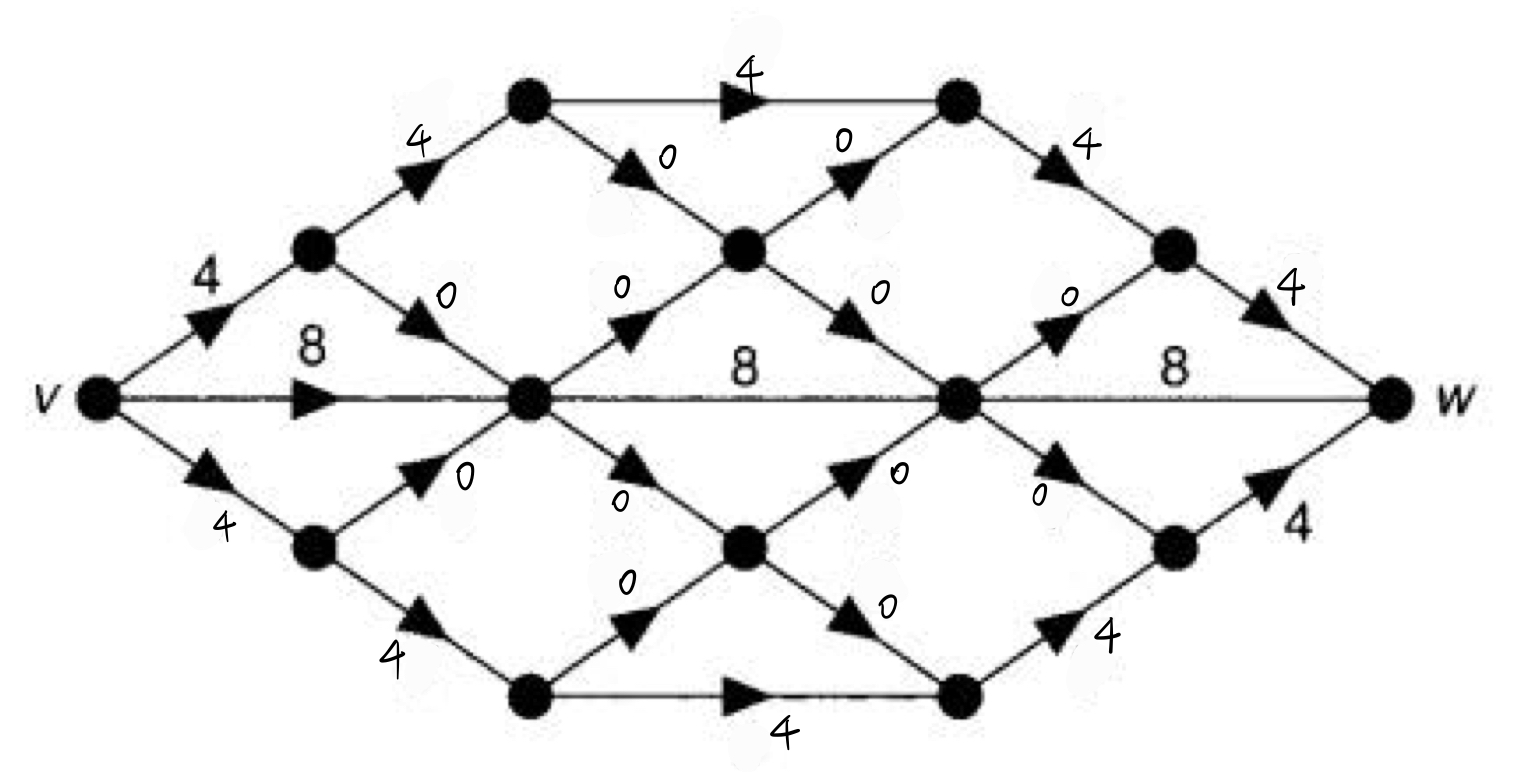
\includegraphics[width=0.8\columnwidth]{Figure/Fig4.jpg}
			\caption{Flow with value 20.}
			\label{fig:4}
		\end{figure}
		
		Since the network has a cut of capacity 20, this flow is a maximum flow and the cut is a minimum cut.
	\end{solution}
	
	\begin{problem}
		(Exercise 6.22)
		
		\begin{enumerate}[(i)]
			\item Consider a network with several sources and sinks. Show how the analysis of the flows in this network can be reduced to the standard case by the addition of a new ‘source vertex’ and ‘sink vertex’.
			\item Illustrate your answer to part (i) with reference to the network in Fig. \ref{fig:5}.
			\begin{figure}[H]
				\small
				\centering
				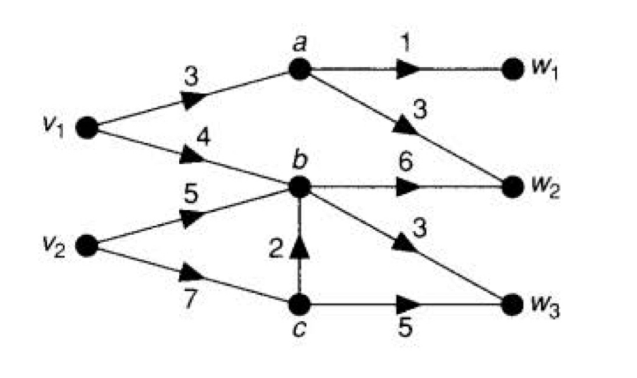
\includegraphics[width=0.5\columnwidth]{Figure/Fig5.png}
				\caption{Figure for Problem 4.}
				\label{fig:5}
			\end{figure}
		\end{enumerate}
		
	\end{problem}
	
	\begin{solution}
	\begin{enumerate}[(i)]
		\item Add a new source vertex \( v^* \) joined to all the sources \( v_i \) with arcs \( v^*v_i \) of infinite capacity,  
		and a new sink vertex \( w^* \) joined to all the sinks \( w_i \) with arcs \( w_iw^* \) of infinite capacity.
		\item See Fig. \ref{fig:6} .
		\begin{figure}[H]
			\small
			\centering
			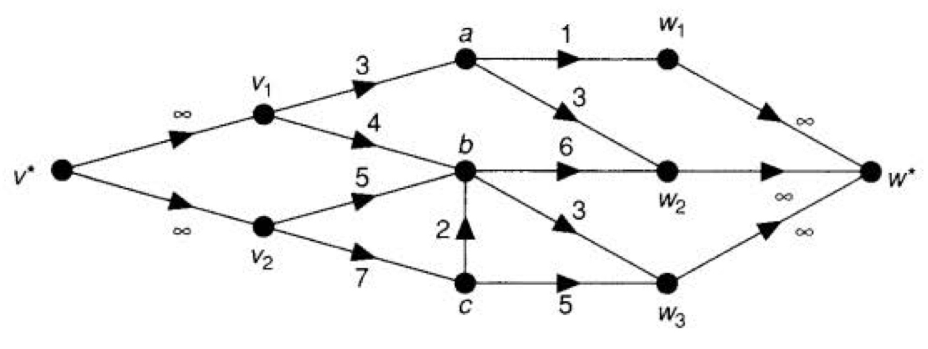
\includegraphics[width=0.5\columnwidth]{Figure/Fig6.png}
			\caption{Solution for Problem 4.}
			\label{fig:6}
		\end{figure}
	\end{enumerate}
	
		
	\end{solution}
	
	\begin{problem}
		(Exercise 6.23)
		
		\begin{enumerate}[(i)]
			\item Use the marriage condition to show that if each girl has \( r \, (\geq 1) \) boy friends and each boy has \( r \) girl friends, then the marriage problem has a solution.
			
			\item Use the result of part (i) to prove that, if \( G \) is a bipartite graph which is regular of degree \( r \), then \( G \) has a complete matching. Deduce that the chromatic index of \( G \) is \( r \). \\
			(This is a special case of Theorem 5.18.)
		\end{enumerate}
		
	\end{problem}
	
	\begin{solution}
		
		\begin{enumerate}[(i)]
			\item 
			Let \( G = (X \cup Y, E) \) be a bipartite graph where \( X \) is the set of girls and \( Y \) is the set of boys. Assume:
			\begin{itemize}
				\item Each girl has degree \( r \geq 1 \), i.e., each girl is connected to exactly \( r \) boys.
				\item Each boy also has degree \( r \), i.e., each boy is connected to exactly \( r \) girls.
			\end{itemize}
			
			We now prove that this condition implies Hall's condition, i.e., for every subset \( S \subseteq X \), its set of neighbors \( N(S) \subseteq Y \) satisfies:
			\[
			|N(S)| \geq |S|.
			\]
			
			Let \( S \subseteq X \), with \( |S| = k \). Each girl in \( S \) is connected to exactly \( r \) boys, so the total number of edges leaving \( S \) is:
			\[
			e(S) = r \cdot k.
			\]
			These edges must go to nodes in \( N(S) \subseteq Y \). Since each boy has degree \( r \), each boy in \( N(S) \) can be incident to at most \( r \) of these edges. Thus:
			\[
			e(S) \leq r \cdot |N(S)|.
			\]
			Combining:
			\[
			r \cdot k \leq r \cdot |N(S)| \Rightarrow |S| \leq |N(S)|.
			\]
			
			Therefore, Hall's condition holds, and by Hall's Marriage Theorem, there exists a matching in which each girl is matched to a boy she knows.
			
			\item 			

			If \( G \) is a bipartite graph that is regular of degree \( r \), then each vertex in both parts of the bipartition has degree \( r \). From part (i), we have shown that such a biregular bipartite graph admits a complete matching.
			
			We can now deduce the chromatic index of \( G \).
		    Since \( G \) is \( r \)-regular and bipartite, by K\H{o}nig's Line Coloring Theorem, the chromatic index of \( G \) equals its maximum degree.
		    That is, the edges of \( G \) can be colored using exactly \( r \) colors such that no two adjacent edges share a color.

			Thus, the chromatic index of \( G \) is \( r \).
			
		\end{enumerate}
	
		
	\end{solution}
	
	
	
	
	\begin{problem}
		(Exercise 6.26)
		
		Let \( \mathcal{F} \) be a family consisting of \( m \) non-empty subsets of \( E \), and let \( A \) be a subset of \( E \).
		By applying Hall’s theorem to the family consisting of \( \mathcal{F} \), together with \( |E| - m \) copies of \( E - A \), prove that there is a transversal of \( \mathcal{F} \) containing \( A \) if and only if
		
		\begin{enumerate}
			\item[(i)] \( \mathcal{F} \) has a transversal;
			\item[(ii)] \( A \) is a partial transversal of \( \mathcal{F} \).
		\end{enumerate}	
		
	\end{problem}
	
	\begin{solution}
		
		Let \( \mathcal{F} = \{S_1, S_2, \ldots, S_m\} \) be a family of \( m \) non-empty subsets of a finite set \( E \), and let \( A \subseteq E \). Consider the problem of determining whether there exists a transversal \( T \) of \( \mathcal{F} \) such that \( A \subseteq T \). We will prove that such a transversal exists if and only if (i) \( \mathcal{F} \) has a transversal, and (ii) \( A \) is a partial transversal of \( \mathcal{F} \).
		
		To this end, consider a new family \( \mathcal{F}' \) obtained by augmenting \( \mathcal{F} \) with \( |E| - m \) copies of the set \( E - A \). That is,
		\[
		\mathcal{F}' = \mathcal{F} \cup \{E - A, E - A, \ldots, E - A\} \quad \text{(with } |E| - m \text{ copies of } E - A).
		\]
		We now apply Hall's theorem to the family \( \mathcal{F}' \). Recall that a transversal exists for \( \mathcal{F}' \) if and only if for every subfamily \( \mathcal{G} \subseteq \mathcal{F}' \), we have
		\[
		\left|\bigcup_{S \in \mathcal{G}} S\right| \geq |\mathcal{G}|.
		\]
		
		Suppose there exists a transversal \( T \subseteq E \) of \( \mathcal{F} \) with \( A \subseteq T \). Then \( |T| = m \), and \( T \) intersects each \( S_i \in \mathcal{F} \) in exactly one distinct element. Since \( A \subseteq T \), the elements of \( T - A \) are distinct from those in \( A \), and their count is \( m - |A| \). To extend \( T \) to a transversal of \( \mathcal{F}' \), we may choose \( |E| - m \) additional elements from \( E - A \), which is possible since \( E - A \) has size \( |E| - |A| \) and \( |E| - |A| \geq |E| - m \), because \( |A| \leq m \).
		
		Thus, we can construct a transversal of \( \mathcal{F}' \) by using all the elements of \( T \) (including \( A \)) and additional distinct elements from \( E - A \) to match the added copies of \( E - A \). Hence, the existence of a transversal of \( \mathcal{F} \) containing \( A \) implies that \( \mathcal{F}' \) has a transversal.
		
		Conversely, suppose \( \mathcal{F}' \) has a transversal \( T' \subseteq E \). Since \( \mathcal{F}' \) contains \( m \) original sets from \( \mathcal{F} \) and \( |E| - m \) copies of \( E - A \), the transversal \( T' \) has exactly \( |\mathcal{F}'| = |E| \) elements, and each element of \( T' \) is used to represent one set in \( \mathcal{F}' \). In particular, since the added sets are all equal to \( E - A \), the elements of \( A \) cannot be used to satisfy any of those sets. Therefore, the elements of \( A \) must be used to satisfy sets from \( \mathcal{F} \). Hence, each element of \( A \) must belong to a distinct set in \( \mathcal{F} \), and no two of them satisfy the same set. That is, \( A \) forms a partial transversal of \( \mathcal{F} \). Moreover, the remaining elements of \( T' \) assigned to the sets in \( \mathcal{F} \) outside of those already matched by \( A \) yield a full transversal of \( \mathcal{F} \), ensuring that \( \mathcal{F} \) has a transversal.
		
		Therefore, there exists a transversal of \( \mathcal{F} \) containing \( A \) if and only if (i) \( \mathcal{F} \) has a transversal and (ii) \( A \) is a partial transversal of \( \mathcal{F} \). 
		
	\end{solution}
	
	\begin{problem}
		(Exercise 6.30)
		
		Show how the max-flow min-cut theorem can be used to prove Hall's theorem.
	\end{problem}
	
	\begin{solution}
		Let \( G \) be a bipartite graph with bipartition \( (A, B) \), where \( |A| = n \), and suppose \( G \) satisfies Hall's condition: for every subset \( S \subseteq A \), we have \( |N(S)| \geq |S| \). We aim to prove that there exists a matching in \( G \) that matches every vertex in \( A \) to a distinct vertex in \( B \), i.e., a matching of size \( n \).
		
		We will prove this using the max-flow min-cut theorem. Construct a flow network based on \( G \) as follows:
		
		\begin{itemize}
			\item Add a source vertex \( s \) and a sink vertex \( t \).
			\item Direct an edge from \( s \) to every vertex in \( A \), each with capacity 1.
			\item Direct an edge from each vertex in \( B \) to \( t \), each with capacity 1.
			\item Direct an edge from each \( a \in A \) to every neighbor \( b \in B \) in \( G \), each with capacity 1.
		\end{itemize}
		
		In this directed graph, any integral flow corresponds to a matching in the original bipartite graph: sending one unit of flow along a path \( s \to a \to b \to t \) corresponds to matching \( a \) to \( b \). Therefore, the maximum number of vertex-disjoint such paths (i.e., maximum matching) equals the maximum flow from \( s \) to \( t \).
		
		To prove that there exists a complete matching from \( A \) to \( B \), it suffices to show that the maximum flow in this network is \( |A| \), i.e., one unit of flow from \( s \) to each vertex in \( A \). By the max-flow min-cut theorem, the maximum flow equals the minimum capacity of an \( s \)--\( t \) cut.
		
		Let the minimum cut be a set of vertices consisting of \( T_1 \subseteq A \) and \( T_2 \subseteq B \), such that the cut separates \( s \cup T_1 \cup T_2 \) from the rest of the graph. The capacity of this cut is the sum of the capacities of the edges from \( s \) to \( A - T_1 \) and from \( B - T_2 \) to \( t \), giving
		
		\[
		\text{cut capacity} = |A - T_1| + |B - T_2| = |A| - |T_1| + |B| - |T_2|.
		\]
		
		To minimize the cut, we must minimize this expression. Since the cut separates the graph, there can be no edges from \( T_1 \subseteq A \) to \( B - T_2 \), which means that all neighbors of \( T_1 \) are contained in \( T_2 \). Hence,
		
		\[
		N(T_1) \subseteq T_2 \quad \Rightarrow \quad |T_2| \geq |N(T_1)|.
		\]
		
		If the min-cut capacity is strictly less than \( |A| \), then
		
		\[
		|A| - |T_1| + |B| - |T_2| < |A| \quad \Rightarrow \quad |B| - |T_2| < |T_1|.
		\]
		
		Rewriting,
		
		\[
		|T_2| > |B| - |T_1| \quad \Rightarrow \quad |T_2| < |T_1| \quad \text{(contradiction if } |N(T_1)| < |T_1|).
		\]
		
		Thus, if \( |T_2| < |T_1| \), then \( |N(T_1)| \leq |T_2| < |T_1| \), violating Hall's condition. Hence, by Hall's condition, the min-cut must have capacity at least \( |A| \), and since \( A \) itself forms a trivial cut of capacity \( |A| \), the minimum cut has exactly this value.
		
		By the max-flow min-cut theorem, the maximum flow is then \( |A| \), which corresponds to a matching of size \( |A| \) in \( G \). Therefore, \( G \) has a complete matching from \( A \) to \( B \).
		
	\end{solution}
\end{document}


